% !TEX root = ../main.tex
\section{Числові характеристики випадкових векторів}

\subsection{Математичне сподівання випадкових векторів}
\begin{definition}\index{математичне сподівання!випадкового вектора}
    \emph{Математичним сподіванням $\E{\vec{\xi}}$} 
    випадкового вектора $\vec{\xi}$ називається вектор 
    $\left(\E{\xi_1}, ..., \E{\xi_n}\right)^T$.
\end{definition}
\begin{remark}
    Математичне сподівання випадкового вектора інколи називають
     \emph{центром розсіювання}.
\end{remark}

\noindent \textbf{Способи знаходження:}
\begin{enumerate}
    \item Знайти закони розподілу окремих координат, а далі --- математичні сподівання цих координат.
    \item Знайти математичні сподівання координат одразу.
    Для $\vec{\xi} = (\xi_1, \xi_2)^T$:
    
    $\E\xi_1 = \begin{cases}
        \sum\limits_i \sum\limits_j x_i p_{ij}, & \vec{\xi} \text{ --- ДВВ} \\
        \int\limits_{-\infty}^{+\infty} \int\limits_{-\infty}^{+\infty} x f_{\vec{\xi}}(x,y) dx dy, & \vec{\xi} \text{ --- НВВ}
    \end{cases}$,
    $\E\xi_2 = \begin{cases}
        \sum\limits_j \sum\limits_i y_j p_{ij}, & \vec{\xi} \text{ --- ДВВ} \\
        \int\limits_{-\infty}^{+\infty} \int\limits_{-\infty}^{+\infty} y f_{\vec{\xi}}(x,y) dx dy, & \vec{\xi} \text{ --- НВВ}
    \end{cases}$
    \vspace{0.5em}
    
    В загальному випадку для ДВВ $\E\xi_k = \sum\limits_{i_1, i_2, ..., i_n} (x_k)_{i_k} p_{i_1 i_2 ... i_n}$, де індекс $i_k$ пробігає кількість
    значень, що приймає координата $x_k$,
    для НВВ $\E\xi_k = \int\limits_{-\infty}^{+\infty}...\int\limits_{-\infty}^{+\infty} x_k f_{\vec{\xi}}(\vec{x}) dx_1 ... dx_n$.
\end{enumerate}

\subsection{Мішані початкові та центральні 
            моменти випадкових векторів}
\begin{definition}\index{момент!початковий!мішаний}
    \emph{Мішаним початковим моментом} порядку 
    $k_1+k_2+...+k_n$ 
    $\left(k_i \in \mathbb{N}\right)$
    випадкового вектора 
    $\vec{\xi} = \left(\xi_1, ..., \xi_n\right)^T$
    називається число
    \begin{equation}
        \alpha_{k_1+k_2+...+k_n} = 
        \E{\xi_1^{k_1} \xi_2^{k_2} ... \xi_n^{k_n}}
    \end{equation}
\end{definition}
\begin{remark}
    $\E\xi_1 = \alpha_{1+0+...+0}, \E\xi_2 = \alpha_{0+1+...+0},
    ..., \E\xi_n = \alpha_{0+0+...+1}$.
\end{remark}
\begin{definition}\index{момент!центральний!мішаний}
    \emph{Мішаним центральним моментом} порядку 
    $k_1+k_2+...+k_n$
    $\left(k_i \in \mathbb{N}\right)$ 
    випадкового вектора
    $\vec{\xi} = \left(\xi_1, ..., \xi_n\right)^T$
    називається число
    \begin{equation}
        \beta_{k_1+k_2+...+k_n} = 
        \E{\mathring{\xi}_1^{k_1}
        \mathring{\xi}_2^{k_2}
        ...
        \mathring{\xi}_n^{k_n}}, \text{ де }
        \mathring{\xi_k} = \xi_k - \E\xi_k
    \end{equation}
\end{definition}
\begin{remark}
    Всі центральні моменти 1-го порядку --- 
    нульові.
\end{remark}
Центральні моменти порядку $0+...+0+2+0+...+0$ --- це дисперсії відповідних координат:
    $$\forall k = \overline{1,n}: 
    \beta_{0+...+0+\underset{k}{2}
    +0+...+0} = \E\mathring{\xi}_k^2 = 
    \D\xi_k$$

Дисперсії координат задають розсіювання 
вздовж відповідних координатних осей.

\begin{definition}\index{момент!кореляційний}\index{коваріація}
    \emph{Кореляційним моментом} або 
    \emph{коваріацією} випадкових величин 
    $\xi_i$ та $\xi_j$ називається мішаний 
    центральний момент 
    порядку
    $0+...+0+\underset{i}{1}+0+...+0+\underset{j}{1}+0+....+0$:
    \begin{equation*}
        {cov}(\xi_i,\xi_j) = \K\xi_i\xi_j = \beta_{0+...+0+\underset{i}{1}+0+...
        +0+\underset{j}{1}+0+...+0}
        =
        \E(\xi_i-\E\xi_i)(\xi_j-\E\xi_j)
    \end{equation*}
\end{definition}
\begin{remark}
    ${cov}(\xi_k, \xi_k) = \E(\xi_k-\E\xi_k)^2 = \D\xi_k$.
\end{remark}
\begin{definition}\index{матриця!кореляційна}
   \emph{Кореляційною матрицею} випадкового 
   вектора $\vec{\xi}$ називається матриця, у яку зібрано усі 
   кореляційні моменти випадкового вектора
   \begin{equation*}
       \K\vec{\xi} = 
       \begin{pmatrix}
           \D\xi_1 & \K\xi_1\xi_2 & \cdots & \K\xi_1\xi_n \\
           \K\xi_1\xi_2 & \D\xi_2 & \cdots & \K\xi_2\xi_n \\
           \vdots & \vdots & \ddots & \vdots \\
           \K\xi_1\xi_n & \K\xi_2\xi_n & \cdots & \D\xi_n
       \end{pmatrix}
   \end{equation*} 
\end{definition}
\begin{remark}
    $\mathring{\vec{\xi}} = \left(\mathring{\xi_1}, ..., \mathring{\xi_n}
    \right)^T$.
    Тоді $\K\vec{\xi} = \E\,\mathring{\vec{\xi}}\,\mathring{\vec{\xi}}^T = \E \left(\vec{\xi} - \E\xi\right)\left(\vec{\xi} - \E\xi\right)^T$,
    де математичне сподівання від матриці $\left(\vec{\xi} - \E\xi\right)\left(\vec{\xi} - \E\xi\right)^T$ визначається поелементно.
\end{remark}

\noindent \textbf{Властивості кореляційного моменту:}
\begin{enumerate}
    \item $\K\xi_i\xi_j = \K\xi_j\xi_i$.
    \begin{proof}
        Випливає з означення кореляційного моменту.
    \end{proof}
    \item Нехай $\eta_1 = a_1\xi_1 + b_1$, $\eta_2 = a_2\xi_2 + b_2$.
    Тоді $\K\eta_1\eta_2 = a_1a_2\K\xi_1\xi_2$.
    \begin{proof}
        $\K\eta_1\eta_2 = \E(\eta_1 - \E\eta_1)(\eta_2 - \E\eta_2) = 
        \E(a_1\xi_1 + b_1 - \E(a_1\xi_1 + b_1))
        (a_2\xi_2 + b_2 - \E(a_2\xi_2 + b_2)) = 
        \E a_1(\xi_1 - \E\xi_1)a_2(\xi_2 - \E\xi_2) = 
        a_1a_2\E(\xi_1 - \E\xi_1)(\xi_2 - \E\xi_2) = 
        a_1a_2\K\xi_1\xi_2$.
    \end{proof}

    \item Зручна формула для обчислення кореляційного моменту.
    \begin{equation}
        \K\xi_1\xi_2 = \E\xi_1\xi_2 - \E\xi_1 \E\xi_2
    \end{equation}
    \begin{proof}
        $\K\xi_1\xi_2 = \E(\xi_1 - \E\xi_1)(\xi_2 - \E\xi_2) = 
        \E(\xi_1\xi_2 - \xi_1\E\xi_2 - \xi_2\E\xi_1 + \E\xi_1\E\xi_2) = 
        \E\xi_1\xi_2 - \E\xi_1\E\xi_2 - \E\xi_2\E\xi_1 + \E\xi_1\E\xi_2 = 
        \E\xi_1\xi_2 - \E\xi_1\E\xi_2$
    \end{proof}
    
    \item $\D(a\xi_1 \pm b\xi_2) = a^2\D\xi_1 \pm 2ab\K\xi_1\xi_2 + 
    b^2\D\xi_2$.

    \begin{proof}
        $\D(a\xi_1 \pm b\xi_2) = 
        \E(a\xi_1 \pm b\xi_2 - \E(a\xi_1 \pm b\xi_2))^2 =
        \E(a(\xi_1-\E\xi_1)\pm b(\xi_2 - \E\xi_2))^2 = 
        a^2 \E\mathring{\xi}_1^2 \pm 2ab\E\mathring{\xi}_1\mathring{\xi} _2 
        + b^2 \E\mathring{\xi}_2^2 = 
        a^2\D\xi_1 \pm 2ab\K\xi_1\xi_2 + b^2\D\xi_2$.
    \end{proof}

    \item\label{cov_ineq} $\left|\K\xi_1\xi_2\right| \leq \sigma_{\xi_1} \sigma_{\xi_2}$. \index{нерівність!Коші-Буняковського}
    \begin{proof}
        Два способи: 
        \begin{enumerate}[label=\Roman*.]
            \item $\D(x\xi_1 \pm \xi_2) = x^2 \D\xi_1 \pm 2x\K\xi_1\xi_2 + \D\xi_2 \geq 0 
            \Rightarrow 4(\K\xi_1\xi_2)^2 - 4\D\xi_1\D\xi_2 \leq 0 
            \Rightarrow $

            $\left|\K\xi_1\xi_2\right| \leq \sigma_{\xi_1} \sigma_{\xi_2}$.

            \item Введемо нормовані центровані випадкові величини $\xi_H = \frac{\xi - \E\xi}
            {\sigma_\xi}$, $\E\xi_H =0$, $\D\xi_H = 1$.

            $\E(\xi_{1H} \pm \xi_{2H})^2 \geq 0 \Leftrightarrow 
            \E(\xi^2_{1H}\pm2\xi_{1H}\xi_{2H}+\xi^2_{2H}) \geq 0 
            \Leftrightarrow 2 \pm 
            2\frac{\K\xi_1\xi_2}{\sigma_{\xi_1}\sigma_{\xi_2}} \geq 0 
            \Leftrightarrow $

            $\left|\K\xi_1\xi_2\right| \leq \sigma_{\xi_1} \sigma_{\xi_2}$.
        \end{enumerate}
    \end{proof}
    \item Якщо $\xi_1$ та $\xi_2$ --- незалежні, то $\K\xi_1\xi_2 = 0$.
    \begin{proof}
        Нехай $\xi_1$ та $\xi_2$ --- незалежні.

        $\K\xi_1\xi_2 = \E\xi_1\xi_2 - \E\xi_1\E\xi_2 = 
        \iint\limits_{\mathbb{R}^2} xy f_{\vec{\xi}}(x,y)dx dy 
        - \E\xi_1\E\xi_2
        = \int\limits_{-\infty}^{+\infty}xf_{\xi_1}(x)dx \cdot
        \int\limits_{-\infty}^{+\infty}yf_{\xi_2}(y)dy
        - \E\xi_1\E\xi_2 = 
        \E\xi_1\E\xi_2 - \E\xi_1\E\xi_2 = 0$.
    \end{proof}

    Обернене твердження, взагалі кажучи, не має місця. Тому випадкові 
    величини, для яких $\K\xi_1\xi_2 = 0$, називаються 
    \emph{некорельованими}. \index{випадкова величина!некорельовані величини}
\end{enumerate}

\begin{example} З некорельованості не випливає незалежність.
    
    \begin{tabular}{c p{10cm}}
        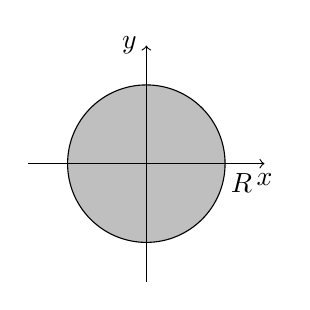
\begin{tikzpicture}[baseline={(current bounding box.north)}]
            \draw [fill = lightgray] (0, 0) circle [radius = 1];
            \draw [->] (-1.5, 0) -- (1.5, 0);
            \draw [->] (0, -1.5) -- (0, 1.5);
            \node [below right] at (0.95, 0) {$R$};
            \node [below] at (1.5, 0) {$x$};
            \node [left] at (0, 1.5) {$y$};
        \end{tikzpicture} &
        Нехай $S = \left\{(x,y) \in \mathbb{R}^2 : x^2 + y^2 \leq R^2\right\}$ і $\vec{\xi} \sim \mathrm{U}(S)$.
        Щільність розподілу дорівнює
        \begin{center}
            $f_{\vec{\xi}}(x, y) = 
            \begin{cases}
            \frac{1}{\pi R^2}, & (x, y) \in S \\
            0, & (x, y) \notin S
        \end{cases}$
        \end{center}
        Знайдемо маргінальні щільності розподілу та відповідні математичні сподівання.
    \end{tabular}

\begin{tabular}{c c}
    $f_{\xi_1}(x) = 
        \begin{cases}
            \int\limits_{-\sqrt{R^2 - x^2}}^{\sqrt{R^2 - x^2}} \frac{1}{\pi R^2} dy
            = \frac{2\sqrt{R^2-x^2}}{\pi R^2},& |x| \leq R \\
            0, & |x| > R
        \end{cases}
    $,
    &
    $f_{\xi_2}(y) = 
    \begin{cases}
        \frac{2\sqrt{R^2-y^2}}{\pi R^2},& |y| \leq R \\
        0, & |y| > R
    \end{cases}
    $
\end{tabular}

$\E\xi_1 = \E\xi_2 = \int\limits_{-R}^R t\cdot\frac{2\sqrt{R^2-t^2}}{\pi R^2} dt = 0$, бо інтегрується непарна функція по симетричному проміжку.

$\K\xi_1\xi_2 = \iint\limits_S xy \frac{1}{\pi r^2} dx dy - \E\xi_1\E\xi_2 =
\frac{1}{\pi R^2}\int\limits_0^{2\pi} d\varphi \int\limits_0^R r^2 \cos \varphi \sin \varphi r dr = 
\frac{1}{2\pi R^2}\int\limits_0^{2\pi} \sin 2\varphi d\varphi \int\limits_0^R r^3 dr = 0$.
Отже, $f_{\vec{\xi}}(x,y) \neq f_{\xi_1}(x)f_{\xi_2}(y)$ і координати вектора залежні, але $\K\xi_1\xi_2 = 0$.
\end{example}

\subsection{Коваріація як скалярний добуток випадкових величин}
Зафіксуємо ймовірнісний простір $\left\{\Omega, \mathcal{F}, \P\right\}$.
Позначимо $\mathcal{L}^2(\Omega) = \left\{\xi : \Omega \rightarrow \mathbb{R} \;|\; \E\xi^2 < +\infty\right\}$.
Оскільки $\D\xi = \E\xi^2 - (\E\xi)^2 \geq 0$, то для $\xi \in \mathcal{L}^2(\Omega)$ $|\E\xi| < +\infty$.
Таким чином, для будь-яких $\xi, \eta \in \mathcal{L}^2(\Omega)$ 
існує ${cov}(\xi,\eta)$, бо $|{cov}(\xi,\eta)| \leq \sqrt{\D\xi} \cdot \sqrt{\D\eta}$.

Для коваріації маємо 
${cov}(a\xi_1 + b\xi_2,\eta) = \E(a\xi_1+b\xi_2)\eta - \E(a\xi_1 + b\xi_2)\E\eta = 
a \E\xi_1\eta + b \E\xi_2\eta - a \E\xi_1 \E\eta - b \E\xi_2 \E\eta = a\cdot{cov}(\xi_1,\eta) + b\cdot{cov}(\xi_2,\eta)$.
Також було доведено ${cov}(\xi, \eta) = {cov}(\eta, \xi)$ та ${cov}(\xi, \xi) \geq 0$.
Виконуються всі умови скалярного добутку, окрім ${cov}(\xi, \xi) = 0 \Rightarrow \xi = 0$.
Ця умова буде виконуватися, якщо розглядати інший простір випадкових величин:
$\mathcal{L}_0^2(\Omega) = \left\{\xi : \Omega \rightarrow \mathbb{R} \;|\; \E\xi = 0, \E\xi^2 < +\infty\right\}$.
\begin{remark}
    Якщо $\xi \in \mathcal{L}^2(\Omega)$, то $\mathring{\xi} \in \mathcal{L}_0^2(\Omega)$.
\end{remark}
\begin{exercise}
    Перевірити, що $\mathcal{L}_0^2(\Omega)$ є лінійним підпростором $\mathcal{L}^2(\Omega)$.
\end{exercise}

\noindent \textbf{Висновок:} ${cov}(\xi, \eta)$ задає \emph{скалярний добуток} на $\mathcal{L}_0^2(\Omega)$.

\vspace{0.5em} \index{нерівність!Коші-Буняковського}
Таким чином, властивість $|{cov}(\xi,\eta)| \leq \sqrt{\D\xi} \cdot \sqrt{\D\eta}$ ---
це нерівність Коші-Буняковського, а кореляційна матриця $\K$ --- це матриця Грама системи
випадкових величин $\left\{\xi_1, \xi_2, ..., \xi_n\right\}$.
З курсу лінійної алгебри відомо, що якщо ці випадкові величини лінійно незалежні, то матриця $\K$ є додатно визначеною, 
і невід'ємно визначеною в загальному випадку.

\subsection{Коефіцієнт кореляції}
\begin{definition}\index{коефіцієнт кореляції}
    \emph{Коефіцієнтом кореляції} називають безрозмірну числову характеристику
    \begin{equation*}
        \rho_{\xi_1\xi_2} = \frac{\K\xi_1\xi_2}{\sigma_{\xi_1}\sigma_{\xi_2}}
    \end{equation*}
\end{definition}

\begin{definition}\index{матриця!кореляційна!нормована}
    Всі коефіцієнти кореляції збираються в 
    \emph{нормовану кореляційну матрицю}:

    \begin{equation*}
        R = 
        \begin{pmatrix}
            1 & \rho_{\xi_1\xi_2} & \cdots & \rho_{\xi_1\xi_n} \\
            \rho_{\xi_1\xi_2} & 1 & \cdots & \rho_{\xi_2\xi_n} \\
            \vdots & \vdots & \ddots & \vdots \\
            \rho_{\xi_1\xi_n} & \rho_{\xi_2\xi_n} & \cdots & 1
        \end{pmatrix}
    \end{equation*}

\end{definition}

\noindent \textbf{Властивості коефіцієнту кореляції:}
\begin{enumerate}
    \item Для некорельованих випадкових величин $\xi_1$ та $\xi_2$ 
    $\rho_{\xi_1\xi_2} = 0$.
    \begin{proof}
        Випливає з означення коефіцієнта кореляції.
    \end{proof}
    \item $\left|\rho_{\xi_1\xi_2}\right| \leq 1$.
    \begin{proof}
        Випливає з властивості \refeq{cov_ineq} кореляційного моменту.
    \end{proof}
    \item $\left|\rho_{\xi_1\xi_2}\right| = 1 \Leftrightarrow 
    \exists \; a, b \in \mathbb{R}: \xi_2 = a\xi_1 + b$.
    \begin{proof}
        Нехай 
        $\xi_2 = a\xi_1 + b$. $\K\xi_1\xi_2 = 
        a\D\xi_1$
        , 
        $\sigma_{\xi_2} = \sqrt{\D\xi_2} = \sqrt{a^2\D\xi_1} = 
        |a|\sqrt{\D\xi_1}$.

        Тоді $\rho_{\xi_1\xi_2} = \frac{a\D\xi_1}{|a|(\sqrt{\D\xi_1})^2} 
        \Rightarrow
        \left|\rho_{\xi_1\xi_2}\right| = 1$.

        Нехай $\left|\rho_{\xi_1\xi_2}\right| = 1$.
        $\E\left(\frac{\xi_1 - \E\xi_1}{\sigma_{\xi_1}} 
        \pm \frac{\xi_2 - \E\xi_2}{\sigma_{\xi_2}}\right)^2 = 
        2(1\pm\rho_{\xi_1\xi_2}) = 0$.

        $\E\xi^2 = 0 \Rightarrow \D\xi = -(\E\xi)^2 \geq 0 \Rightarrow \begin{cases}
            \E\xi = 0 \\ \D\xi = 0
        \end{cases} \Rightarrow \xi$ приймає значення $0$ з ймовірністю $1$.

        Отже, $\frac{\xi_1 - \E\xi_1}{\sigma_{\xi_1}} 
        \pm \frac{\xi_2 - \E\xi_2}{\sigma_{\xi_2}} = 0$ з ймовірністю $1$,
        звідки отримуємо лінійний зв'язок.
    \end{proof}
\end{enumerate}
\begin{example}
    Скласти кореляційну та нормовану кореляційні матриці випадкового вектора $\vec{\xi} = (\xi, \eta)^T$,
    який рівномірно розподілений в еліпсі $D = \left\{(x, y) : \frac{x^2}{4} + \frac{y^2}{9} \leq 1 \right\}$.

    Оскільки площа цього еліпса дорівнює $6\pi$, то щільність розподілу має вигляд
    \begin{gather*}
        f_{\vec{\xi}}(x, y) = \begin{cases}
            \frac{1}{6\pi}, & (x, y) \in D \\
            0, & (x, y) \notin D
        \end{cases}
    \end{gather*}
    Внаслідок симетрії області $D$ відносно початку координат $\E\xi = \E\eta = 0$.
    Знайдемо дисперсії обох координат:
    \begin{gather*}
        \D\xi = \frac{1}{6\pi} \iint\limits_D x^2 dx dy =
        \left[ \begin{gathered}x = 2 r\cos\varphi \\ y = 3 r\sin\varphi \\ |\mathcal{J}| = 6r\end{gathered}\right] =
        \frac{1}{\pi} \int\limits_0^{2\pi}\cos^2 \varphi d\varphi \int_0^1 4 r^3 dr =
        \frac{1}{\pi} \cdot \pi \cdot 1 = 1
    \end{gather*}
    Аналогічно
    \begin{gather*}
        \D\eta = \frac{1}{6\pi} \iint\limits_D y^2 dx dy =
        \frac{1}{\pi} \int\limits_0^{2\pi}\sin^2 \varphi d\varphi \int_0^1 9 r^3 dr =
        \frac{1}{\pi} \cdot \pi \cdot \frac{9}{4} = \frac{9}{4} 
        \\
        \K\xi\eta = \frac{1}{6\pi}\iint\limits_D xy dx dy = 
        \frac{1}{\pi} \int\limits_0^{2\pi} \cos\varphi \sin\varphi d\varphi \int_0^1 6 r^3 dr = 0
    \end{gather*}
    Отже, кореляційна та нормована кореляційна матриці мають вигляд
    \begin{gather*}
        \K = \begin{pmatrix}
            1 & 0 \\
            0 & 2.25
        \end{pmatrix}, \;
        R = \begin{pmatrix}
            1 & 0 \\
            0 & 1
        \end{pmatrix}
    \end{gather*}
\end{example}